\newpage
%%%%%%%%%%%%%%%%%%%%%%%%%%%%%%%%%%%%%%%%%%%%%%%%%%%%%%%%%%%%%%%%%%%%%%%%%%%%%%%
\section{Week 7?}
%%%%%%%%%%%%%%%%%%%%%%%%%%%%%%%%%%%%%%%%%%%%%%%%%%%%%%%%%%%%%%%%%%%%%%%%%%%%%%%
\subsection*{Saturday, 04/20/2024}
\begin{itemize}
    \item \textcolor{blue}{\href{https://github.com/queazyg}{Q}} is helping me with ai nyt server.
    \item I am hard stuck on messages so perhaps we will crack it together.
\end{itemize}

\subsection*{Sunday, 04/21/2024}
\begin{itemize}
    \item Got diesel initialized in the project for storing articles, have not
        yet tested the ORM yet, I'll do this soon. 
    \item I was distracted by the reactions feature for the network times. This
        was really easy to add, and I styled it indigo-300 or something like
        this. I've never seen a social site have this color like, so it's
        interesting at least.
    \item You can't yet press the like, this will work once I finally figure out
        how to make the app a valid signer for users.
    \item I added a profile page as shown in Figure~\ref{fig:pfp_page}.
        \begin{figure}[ht]
            \centering
            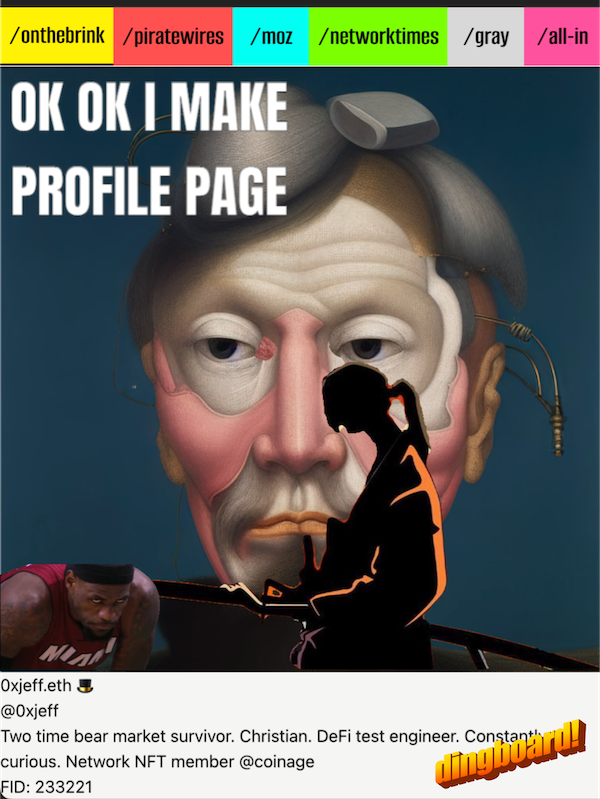
\includegraphics[width=7cm]{pfp_page}
            \captionsetup{labelfont=bf, textfont=it}
            \caption{Profile Page}
            \label{fig:pfp_page}
        \end{figure}
    \item I added hover effects (you can't see it here but matt's pfp background
        has a slight black circle with 10\% opacity applied here
        (Figure~\ref{fig:hover_pfp}).
        \begin{figure}[ht]
            \centering
            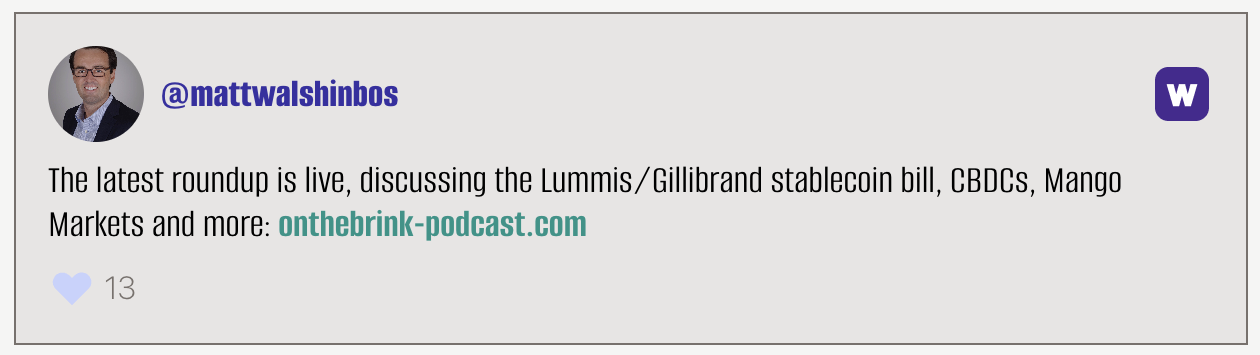
\includegraphics[width=9cm]{hover_pfp}
            \captionsetup{labelfont=bf, textfont=it}
            \caption{Pfp Hover Effect}
            \label{fig:hover_pfp}
        \end{figure}

\end{itemize}

